First week in China (introduction vinnete):
- ``rou'': mysterious carnal sport --> social community
- XNT fall from grace:
- Qingdao:
    - basketball (actionScrutiny)
    - Asia 7s: (Qi gaige & Li sheng) (system, incentives)
    - National 7s: Beijing:WCY out of the huddle


XNT:
- Sport as a upward mobility strategy:
    - Many from athletics (IND) to rugby (TEAM)
- Fall from grace --> Lack of click?
- System: coach ()
- Zero to one: new comers, uni students, senior players, old motherlandStrength

In this system, how do they interaction

%%%%%%%%%%%%%%%%%%%%%%%%%%%%%%%%%%%%%%%%%%%%%%%%%%%%%%%%%%%%%%%%%%%%%%%%%%%%%%%%%%%%%%
ABSTRACT:
Fieldwork in Beijing


First Week in Beijing:

The night after I arrived in Beijing in late August 2015, I was invited to a dinner hosted by Adrian, an elder of the Chinese rugby community in Beijing.  Adrian was the captain of the second graduating class of rugby players the Chinese Agricultural University (CAU), the home of China's first official rugby union program established in 1990.  I first met Adrian two years earlier in 2013, through a good friend Kai. Kai was  a more recent CAU graduate, a former Chinese National rugby team representative, and now a lawyer in Beijing.  Kai was also invited to the dinner, as was Mr Shi, a sports television producer from Chinese Central Television (CCTV).  The background to the dinner was that World Rugby, the international governing body of rugby, had recently given CCTV the broadcasting rights to the 2015 Rugby World Cup, to be held imminently in England during September and October 2015.  Mr Shi had been charged with the production of the 48-match tournament, which would be the first time international rugby was televised on Chinese national television.  Mr Shi was completely new to rugby, and so needed help making rugby accessible and understandable for Chinese audiences.  Shi tracked down Adrian, and Adrian in turn tracked down Kai.  Both Adrian and Kai were
well connected to the Chinese rugby community and fluent in English, and so were well placed to assist Mr Shi in the tasks of translating relevant rugby materials and organising expert commentators for the broadcast. My arrival in Beijing was timely for this project, and so Kai was quick to recruit me to join them at dinner.  I was eager to begin my fieldwork and so, despite my mild to moderate jet lag accepted the invitation and set off to the restaurant with my notepad and audio recorder in hand.

\subsection{My history with rugby and China (Qualifications of the researcher)}
It had been two years since I had last spent a long period of time in China, the last time being in 2013 when I spent eight months coaching the Chinese men's youth rugby 7s team in the lead up to the Nanjing Asian Youth Olympics.  Before that, I had spent one year studying on Exchange at Beijing University in 2008, and another year before that on an intensive Chinese language course at Liaoning University, Shenyang, in 2006.  Rugby featured heavily in both instances.  In 2006, an Australian classmate and friend Ed had caught wind of the fact that there was a rugby program down the road from Liaoning University at the Shenyang Sports College (SSC).  Despite the fact that we had both been diligently attending class and courageously deploying our elementary Chinese to order food at restaurants and befriend local taxi drivers, Ed and I were, nonetheless, three months into our intensive language exchange and feeling that our Chinese skills were floundering.  We suspected that this was in large part due to the fact that we had met very few local Chinese people our age.  So one afternoon we rode our bikes over to the Shenyang Sports College in time for the rugby team's afternoon training session.  Less than six months later, we were boarding an overnight train from Shenyang to Shanghai with the SSC rugby team to compete in the annual Shanghai Rugby 7s Tournament.  We had become closely integrated into the community of rugby athletes at SSC, due in part to the common language of rugby that we all shared, and perhaps mostly due to the overwhelming hospitality of the SSC rugby team.  The decision to find the rugby team may have also helped us improve our Chinese. Ed and I were the only two in our cohort to finish the year in Shenyang with a Level 6 in the Chinese Proficiency Exam, which qualified us to study alongside Chinese local students at an undergraduate level.

Buoyed by this experience with the SSC rugby team in 2006, I followed a similar template two years later when I arrived in Beijing on exchange from Sydney University to study sociology at Beijing University.  At that time in Beijing, the only Chinese rugby program was based out of the Chinese Agricultural University, a forty minute cycle north of Beijing University.  It was during my time training and generally ``hanging out'' at CAU that I met and developed a strong friendship with Kai, who was at the time playing for CAU and China, while also finishing a Master's degree in Labour Law.  I also met and developed relationships with many rugby players, coaches, and general fans of the Beijing rugby community.  The CAU rugby program was the strongest in the country: CAU consistently outperformed its rivals at the time (Shanghai Sports Institute, the People's Liberation Army, and SSC) and it was awarded with the responsibility of hosting the Chinese national team.  When the International Olympic Committee announced in late 2009 that rugby would be played in the 2016 Rio De Janeiro Olympics, it was subsequently decided in 2010 that rugby would be inducted into the the state sponsored sports system and played in the next Chinese National Games in 2013.  Following this announcement, many of CAU's athletes and coaches dispersed to various professional provincial rugby programs, the main ones being Beijing and Shandong.

Between 2009 and 2013 I returned to Australia to finish my undergraduate degree, during which time my own rugby career also rapidly developed. After a successful season in the Sydney premiership competition in 2009, I was selected to play for the Australian Rugby Sevens team. I represented Australia in Sevens from 2009 through to the end of 2012.  In 2013, during the 9 month gap between my Australian rugby contract ending and the start of my graduate studies at Oxford University, I returned to China to coach the Chinese Youth Men's 7s program in their lead-up to the 2013 Nanjing Asian Youth Olympics.  Along with a small team of Chinese coaches and management, I coached a core group of roughly 25 athletes aged between 15 and 18 years old. Our athletes trained 6 days a week for approximately 6 months, with only occasional breaks for National holidays, or for athletes to return to their home provinces to complete compulsory exams.  The program was based predominantly in Anhui province, and we travelled from Anhui to other provinces further afield to find suitable practice opportunities against provincial programs.  Soon after the completion of the Asian Youth Olympics in Nanjing, the Chinese National Games were held in Shenyang. Rugby was played for the first time in National Games history, with dramatic consequences.

The Dinner:
Adrian, Kai, and I waited for Mr Shi to arrive in the upstairs area of the Korean BBQ restaurant in a quiet Peking willow lined street just inside Beijing's East 4th Ring Road.  Adrian, as host and elder, held the floor as we waited: he reminisced fondly about his time playing rugby at CAU as well as his time in Beijing after graduating, when he played with the Beijing Devils, a predominantly expat rugby club in Beijing:

  ``Rugby was so much fun in those days, not like today (in the professional era of Chinese rugby).  Everyone was scraping together the money to go on tour, for the love of the game, not for any other reason.''

When Mr Shi finally arrived, Adrian continued the nostalgic story telling mode but naturally shifted his target audience from Kai and me to Mr Shi.  When describing in rich detail the experience of participating in an overseas rugby tour with the Beijing Devils, he interrupted his own story with an explanatory aside directed at Mr Shi, accommodating for the fact that Mr Shi was relatively unacquainted with the sport: ``This sport, rugby union, it's actually very mysterious. If you haven't played it yourself you might not know this type of feeling,'' Adrian respectfully suggested to Mr Shi. ``Because rugby, you know, you're on the field playing together, there's body contact...'' he paused to find the right phrasing,  ``...its a very ``carnal'' type of feeling. Everyone is very close.'' His gesticulating had led him to have both of his hands clenched as fists in front of him like they were cradling a rugby ball, a lit cigarette smouldering between the index and middle finger of his right hand.  Adrian concluded by reiterating: ``Its very mysterious,'' shaking his head as if baffled and releasing his clenched fists to dab the ash from his cigarette into the ashtray in front of him. He took another drag and   finally added,``So it means this rugby ``circle'' here in China is very tight...'' (Circle (quanzi) is a common way to refer to a social group or community of people) ``...but it doesn't mean that its not also a (political) mess!'' The wisdom in this final note was confirmed with a knowing chuckle from all of us, including Mr Shi.

%英式橄榄球这个项目其实特别神秘,没玩过的话您可能不知道这种感觉,因为英式橄榄球么,大家在场上有身体接触,是一种``肉''的感觉,大家互相都特别亲,特别神秘。
%所以在橄榄球这个圈子特别亲, 但这不是说这个圈儿也不乱!

I was particularly struck by this snippet of Adrian's monologue, perhaps because it was so soon in to my fieldwork that I had happened upon such a rich description, in which the visceral sensation of playing rugby (rou) was linked conceptually to social closeness (qin) and the broader social cohesion of the rugby community (quanzi).  I did not fully realise it at the time, but Adrian's closing caveat would also be particularly relevant to the coming months of fieldwork with the Beijing provincial rugby team. I would come to experience first hand the complexity beneath Adrian's sarcastic assertion that the social closeness derived from the visceral experience of taking the field with teammates did not necessarily buffer against the (political) messiness of off-field social interactions between individuals within the imagined community of Chinese rugby players.  These interactions were, after all, structured by broader institutionalised incentives and cultural dispositions that existed well beyond and well before the existence of the rugby field in China.

Interestingly, however, I also came to understand the complexity of this statement from a different standpoint to Adrian.  When going looking for evidence of bonding and social closeness in rugby in the Beijing team, I was bombarded with testimonies and rationales for why social cohesion and closeness did not and could not exist.  (Chinese society is too complicated, athletes are not innately motivated to play rugby, etc).  Nonetheless, when I interrogated deeper in to the details of athlete experience of joint action in rugby, I was able to find evidence that the visceral dimensions of rugby were related to processes of social affiliation.

I left that first dinner motivated to investigate these relationships further.  My next stop was Xiannontan Sports Institute (XNT) on Monday morning, where I was scheduled to meet separately with the vice-principal of the school in charge of the rugby program, and the head coach of the Beijing rugby program, former CAU coach, ZPH.



\subsection{Physical activity in Chinese modern history}
The history of sport and exercise in China's modern transformation is, in many fascinating ways, emblematic of that history itself. A torrid period of colonial occupation in the 18th and 19th Centuries left China's intellectual elite to seek the regeneration of China in the form of a modern nation state.  The subsequent introduction in the late 19th Century of an ethics of group membership centred around the activities of the nation-state, required importation \textit{en masse} of novel linguistic, cultural, and social categories and practices from the West and Meiji Japan \citep{Liu1995}.  Throughout the 20th Century, physical culture (\textit{tiyu}) became a primary pedagogical vehicle for fostering an explicit link between the strength of the physical body and the strength of the Chinese nation \cites[32]{Morris2004}[49]{Brownell1995}.  From the initial embrace of the Olympic Games by an urban Chinese elite at the turn of the century, all the way through to Beijing's eventual hosting of the Olympics in 2008, physical culture has provided the means through which new and normative ways of thinking and behaving have been publicly displayed and transmitted.  Inherent in this process has been the tension and interaction between imported modes of group membership fostered by the state (i.e., civil society, citizenship, nationalism), with more local and indigenous understandings of social identity centred on intragroup relational processes rooted in Confucian, rural, and dynastic cultural traditions \citep{Fei1992}.  Physical culture in China choreographs---perhaps more explicitly than any other facet of contemporary Chinese life—--the interaction between imported and traditional modes of group membership at the psychological heart of China's modern history.

Throughout China's modern history, a rich indigenous physical culture merged with modern waves of cultural importation beginning in the mid 19th Century. Modern sport and exercise was first introduced to China as part of the ``New Culture Movement'' at the start of the 20th Century—--a movement in which student intellectuals problematised traditional Daoist and Confucian understandings of the body as ``passive'' and ``feudal,'' and suggested that a new, active and competitive body, should be realised \citep{Ge2005}.  Spenserian ideology celebrated the cultivation of the physical body as foundational to the cultivation of the modern Nation-State \citep{Morris2004}. In this vein, the passive and weak Chinese body of the feudal past was publicly identified by student intellectuals and nationalist political movements as the cause of the China's collective weakness as it grappled with colonialism in the early 20th century.
In its place, a strong, masculine, and active body as was established as a central public representation of China's bright future \citep{Brownell1995}, see Figure ~\ref{fig:motherlandStrength}).  As such, towards the end of the 19th century, traditional practices of self-cultivation such as the Daoist notion of ``cultivating life'' (\textit{yangsheng zhidao}), which included traditional martial practices of taichi and qigong, were denounced by reformers in favour of a variety of imported physical regimes and an associated philosophy of ``training the body'' (\textit{duanlian shenti}, see \cite{Farquhar2012}).  The first recorded organised training of bodies, in a non-Indigenous sense, was in 1895 when the Chinese military adopted calisthenics and military drills as an attempt to modernise practices in line with the German and Japanese armies that occupied Chinese territory \citep[viii]{Knuttgen1990}.
Such techniques were soon popularised within elite intellectual communities as pedagogical tools designed to foster an explicit link between the strength of the physical body and the strength of the Chinese nation \cites[32]{Morris2004}[49]{Brownell1995}.

\begin{figure}[htbp]
  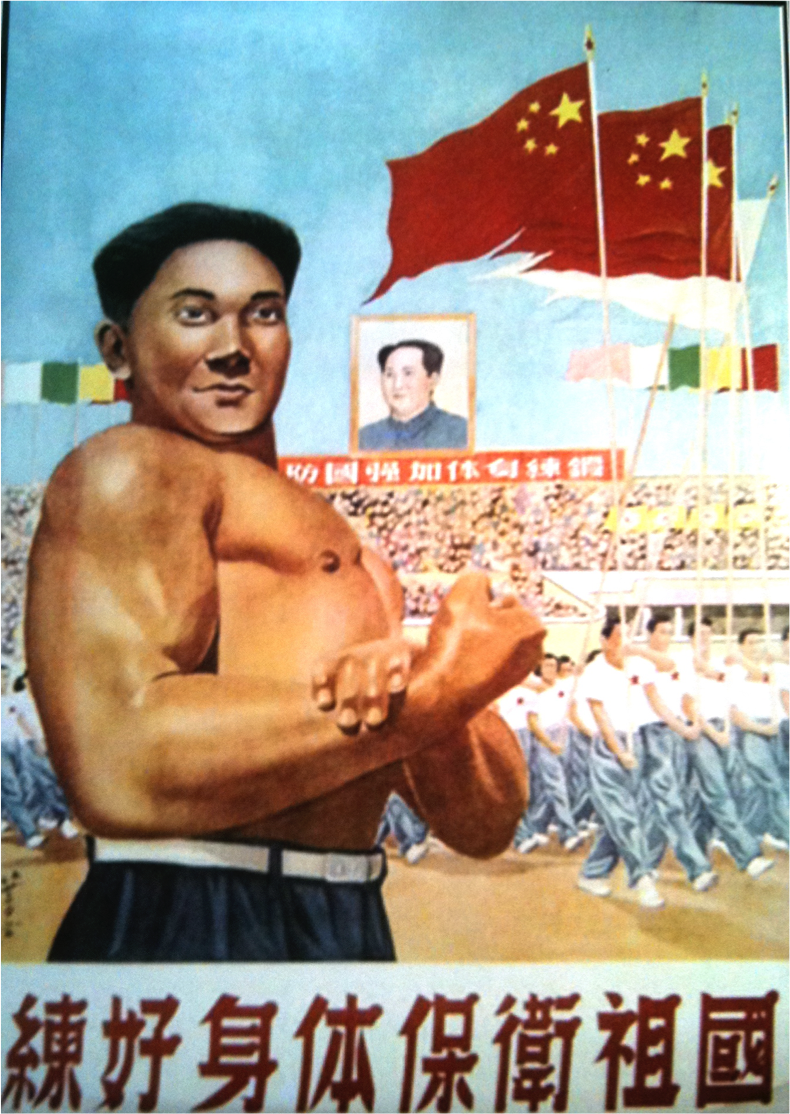
\includegraphics[width = \linewidth]{images/motherlandStrength.png}
  \caption{Strengthen Physique to Defend Motherland (1950)}
  \label{fig:motherlandStrength}
\end{figure}

During this period, China's urban elite began to embrace a range of Anglo-American competitive sports that were promoted by Western missionaries, in particular the YMCA (Young Men's Christian Association).  The YMCA's mission of prescribing Christian manhood for an emerging Chinese youth, including the propagation values of fair play, sportsmanship, masculinity and internationalism, gelled with the values of a nationally (and internationally) motivated urban elite \citep[240]{Morris2004}.  A significant aspect of competitive sports was the fact that they provided a public spectacle, in the form of ``games meets'' (\textit{yundonghui}), in which the performance of emerging national and international political identities could take place \citep{Brownell2008}.
As early as 1908, the Chinese sport community enshrined the Modern Olympic Games as the pinnacle of participation in an international community of nations, and as such, the quadrennial global ritual has since preoccupied Chinese sporting consciousness, and Chinese national consciousness more broadly \cites{Jarvie2008}{Barme2009}[19]{Brownell2008}[3]{Morris2004}{Xu2010}.


SOVIET SYSTEM post 1948
Along with many other facets of Chinese society after 1949, tiyu was institutionalised in line with Soviet bureaucratic models of governance.  In 1952 the “State Sports (and Physical Culture) Commission” (国家体育运动委员会 guojia tiyu yundon wieyuanhui) (hereafter the Sports Commission) was established, which acted as the central State organ responsible for the administration of both “tiyu for the masses” (群众体育 qunzhong tiyu) and “tiyu education” (体育教育 tiyujiaoyu) (tiyu education programs for schools and other institutions), as well as an elite competitive tiyu system (竞技体育体系 jingji tiyu tixi).  The competitive tiyu system was designed to complement “tiyu for the masses” and “tiyu education” by producing model athletes capable of performing and advocating the healthy, egalitarian and militaristic body promoted by the Party (Brownell 1995: 56).   The structure of the tiyu system exists today largely unchanged, although its name changed in 1998 to “The General Administration of Sport in China” (国家体育总局 Guojia tiyu zongju) (hereafter the Sports Administration).

At the bottom of the hierarchical structure are local sports commissions (county, township and city), above which are the provincial and municipal sports commissions; and at the top is the Sports Administration, located in Beijing (Brownell 1995: 59).  The Sports Administration is responsible for all sports training centres and sports programs, of which there are many types.  On one extreme there is the elite professional arm of the Sports Administration, a “national (tiyu) system” (举国体系 juguo tixi), which presides over all full-time professional sports teams (体工队 tigongdui) that exist at national and provincial/municipal levels.  The main objective of this national system is to cultivate elite athletes to compete on a national and international level, in events such as the National Games (全国运动会 Quanguo yundonghui), the Asian Games (亚洲运动会 Yazhou yundonghui), and most importantly, the Olympic games.  Due to an overwhelming Olympic-focus, all sports under the umbrella of professional arm of the Sports Commission are either Olympic sports, or Chinese martial arts (Guojia tiyu zongju 2009a).  Outside of this professional arm, elite tiyu programs are embedded within secondary and tertiary education institutions in a number of different ways, under the banner of the “high school and university tiyu system” (高校体制 gaoxiaotizhi) (Guojia tiyu zongju 2009a).  At a high school level, elite sports programs are offered at “extracurricular sports schools” (业余体校 yeyu tixiao), as well as regular high schools who focus on one or two tiyu programs in particular (Brownell 1995: 59). At a tertiary level, a number of specialist tiyu colleges operate at national, provincial/municipal and local levels.

Reform era sport (1976-1995)
The death of Mao and the end of the Cultural Revolution in 1976 signalled the beginning of widespread social and economic transformations in China, in which the development of the sportsworld was heavily implicated.  Susan Brownell’s work, Training the Body for China (1995), the first and most comprehensive attempt at an anthropology of sport in China, was researched during the mid 1980s at a time when China was only just beginning to interact politically and economically with an international community.  In reference to the unprecedented success of the Chinese women’s volleyball team in the 1980s, Brownell explains how sport functioned as a crucial symbolic practice for China in the process of “rejoining the world” (1995: 86).  As a participant in the tiyu system as a student-athlete herself, Brownell draws on first-hand ethnographic experience of the state-administered “microtechniques of power” (Foucault 1977) that produce the athlete-subject in post-Mao China.  Using two interrelated interpretive frames of “body culture” and “public culture” Brownell interrogates the role of the athlete in the perpetuation of a hyper-visible and “generalisable” politico-moral order—cast in official terms as a “socialist spiritual civilisation” (精神文明 jingshen wenming) (1995: 156).  Brownell explains that the position of the athlete in reform era China is one characterised by the tensions and shifts of an ever-transforming social terrain structured by contradictory forces of the state and the emerging logic of the market.  Although “things have changed”, so to speak, since Brownell’s time of writing, the insights made by Brownell in Training the Body for China provide a solid and invaluable foundation for an anthropology of sport in China.  Indeed, as I argue in this study of rugby in contemporary China, many of the same tensions and contradictions surrounding the athlete that Brownell identifies persist today, only in new and different mutations of experience within the sportsworld.

One of the most immediate transformations to effect the tiyu system, and particularly relevant to the case of rugby in China, was the restoration of the University Entrance Examination (高考 gaokao) (hereafter gaokao), following the end of the Cultural Revolution in 1976 (Brownell 1995: 198).  School curricula were immediately redesigned around the gaokao, and as a result, schools quickly reduced emphases on tiyu programs as they were seen to draw student’s attention and energy away from academic study.  A situation thus emerged where the only option for committed athletes was to attend a specialist sports school in which a scholastic education was not emphasised or was abandoned all together in favour of intense physical training.  Amidst broader social anxieties concerning not only the alarming “quantity” of the Chinese population (人口过多 renkou guoduo), but also the problem of “population quality” (人口素质 renkou suzhi), the widening of the gap between the tiyu and education systems was seen as a “crisis in Chinese sports” (Brownell 1995: 199).  A rise in the public status of the athlete during this same period, due to China’s rejoining of the international sporting community, meant that the social category of the athlete also came under much public scrutiny.  The athlete in China was problematised as lacking sufficient “cultural quality” (文化素质 wenhua suzhi) in accordance with his or her elevated social status as a “representative” (代表 daibiao) of the Chinese nation on an ever-expanding international stage (Guojia tiyu zongju 2009a; Brownell 1995: 95).

The Sports Commission’s response to this crisis was to adopt the policy of “combining sport and education” (体教结合 tijiao jiehe).  Modelled on the US college sports system, beginning in the late 1980s “high level tiyu programs” (高级体育项目 gaoji tiyu xiangmu) were embedded within existing stand alone high schools and universities so as to ensure the “all-round development” (全面发展 quanmian fazhan) of the athlete (Brownell 1995: 203).  As a result, various non-Olympic sports, including rugby, were also inducted into the tiyu system via this channel, as part of an emphasis on a broader range of sports and their perceived potential to facilitate international relations as well as commercial opportunities (Knuttgen, Ma and Wu 1990: 70).  Above all, this relative “democratisation” of the tiyu project was driven by a persistent faith in the ability of tiyu to produce Chinese bodies—now scrutinised based on their inherent “quality” (Woronov 2003: 7).


INCOMPLETE REFORM due to Beijing 2008 performance focus
Stalled reform article: http://www.newschinamag.com/newschina/articleDetail.do?article_id=2409&section_id=15&magazine_id=22


\subsection{Rugby in China}
Although reportedly existing in China within colonial and expatriate circles for more than a century (Reason and Carwyn 1979: 210; HKRFU 2009), and as a modified military exercise as early as the 1930s (Morris 2004: 135), rugby was a late entrant into the Chinese sport system, established as a “high level tiyu programs” in 1990.  The advent of rugby in China can thus be understood in terms of the processes of tiyu “democratisation” explained above.  The introduction of rugby into China was initiated originally at CAU by professor Shi Zhengsheng (施振声) who was introduced to rugby by his supervising professor while completing vocational studies at Azabu University in Japan 1987-1989.  Following Shi’s return to CAU, an exchange relationship was set up between the two universities, and throughout 1990, coaches and referees from Azabu University came to BAU to help set up the necessary infrastructure required for a rugby program.  On the 12th December 1990, China’s first rugby union team was created.  The program was originally made up of existing CAU students who expressed interest in the novel activity, but by its second year, the program earned status as a “high level tiyu program” and was subsequently advertised to student-athletes across the country (Xu 2010: 2).

Based on this original CAU model, rugby programs have since been established within over 30 regular universities and specialist sports colleges in cities throughout China.  A number of rugby clubs (俱乐部 julebu), organisations completely independent of the state sports system, have also begun to spring up in major cities.  Both the men and women’s national teams, made up of players predominantly from CAU, but also from other well-established programs based at the Shanghai Sports University (沈阳体育学院 Shanghai tiyu xueyuan), Shenyang Sports College (沈阳体育学院 Shenyang tiyu xueyuan) and the People’s Liberation Army Sports College (中国人民解放军体育学院 Zhongguo renmin jiefangjun tiyu xueyuan), consistently compete against other nations in the Asia Pacific region (most notably in the Asian Games and the East Asian Games), and are also occasionally involved in top-tier international tournaments such as the International Hong Kong Sevens.

Before rugby became a professional sport in 2010, it had existed as a non-professional university sport for 20 years.  First established in 1990 at CAU, Beijing, rugby was and still is part of a large collection of ``cold-gate'' sports (\textit{lengmen xiangmu}, a term that refers to a profession, trade or branch of learning that receives little attention) in China, with a relatively small participation base compared to other interactive team sports like basketball or football.  While football and basketball have matured as standalone enterprises with supporting market-based consumer industries, most other sports in China (i.e., all other Olympic events, including rugby) exist primarily due to the support of the enormous state-sponsored sport system.  Whereas the commercial basketball and football industries might offer a small percentage of prospective athletes incentives of fame and fortune, the benefits of a state-sponsored sports programs like rugby are more modest.  Chinese youth either gravitate or are ushered by their parents towards sporting careers primarily due to potential life-course opportunities such as access to tertiary education and post-athletic career employment (in the government sports system).  The extent to which an athlete is able to maximise these potential benefits depends on the strength of an athlete's results (\textit{chengji}).
In Olympic sports, the most important measure of a province's success in state-sponsored sporting terms is the National Games, a quadrennial multi-sport event hosted on rotation by provincial capital cities \citep{Hong2002}.  The amount of funding a province and its provincial sporting institutes and programs receive is decided to a large extent by results at the national games.


However, due to the persistent Olympic focus of the Soviet-modelled Chinese competitive professional sports system (\textit{juguo tizhi}), rugby's recently acquired Olympic status means that it is one of 33 sports featured in the all important quadrennial National Games.  Ten of China's collection of 32 provinces and municipalities that participate in the National Games have full time men's and women's rugby programs.



When rugby union was inducted into the state sponsored sports system in 2010, a few Chinese provinces in particular identified a potential opportunity to achieve a beneficial National Games result by heavily investing in this debutant sport.  Beijing's Temple of Agriculture Sports Institute managed to attract a large amount of China's existing rugby talent—---including the unofficially touted ``Emperor'' (Boss) (\citep{huangdi}) of Chinese rugby, national coach Zheng Hongjun—--from where they were previously based at the Chinese Agricultural University, Beijing.  Meanwhile, Shandong province—--a powerhouse in other provincial sports--—succeeded in attracting the majority of the remaining talent, by token of the fact that a large majority of rugby players in China at the time (indeed, a large proportion of athletes more generally) were of Shandong origin.  Importantly, this talent included the Emperor's student come rival coach Lu Xiaohui.  Besides Beijing and Shandong, Jiangsu and Anhui province were strong contenders for the women's gold medal, while the People's Liberation Army (PLA) and Hong Kong in particular were strong contenders for top spot in the men's competition.

Beijing's results leading into the 2013 national games were strongest overall across the men's and women's teams, however the Hong Kong men's and women's teams had only occasionally participated in these tournaments.  In the semi-finals of the National Games, the Beijing men came up against Hong Kong, while the Shandong men played off against the PLA.  Beijing lost to their stronger and more favoured opponents, whereas Shandong beat the PLA.  Meanwhile in the women's league, both Beijing and Shandong advanced to the final.  The stage was set: Beijing, the favourites led by the reigning Emperor of Chinese rugby, would face Shandong, the underdogs lead by the Emperor's cunning apprentice.

The men's final was played first, and in somewhat of an upset, Shandong edged out Hong Kong to win the gold medal by one try.  In the women's final, scores were level until early in the 2nd half when Shandong went ahead by two tries to nil.  At that point, the Beijing women's team, under instruction from their coach Zheng Hongjun, suddenly stopped playing.  After being asked by the referee and match officials to continue, the Beijing women stood firm and refused to play on, forming a huddle on their side of half-way in the middle of the field. Shandong had no choice but to continue to play out the rest of the 2nd half, running in try after try, until the final score at full time was a farcical 71-0.  Shandong was declared victorious, while Beijing called foul play, claiming that the referee had been unfairly adjudicating the match in Shandong's favour.  The details and dramas of this now well-known story in China's sporting history (known as ``Match-striking-gate'') require more detailed development in a format that exists beyond the scope of this particular study. I introduce the story here in order to highlight its implications for my ethnographic research.

The Beijing women's rugby team was the first Beijing team in the 48-year history of the National Games not to receive the ``medal for civilised spirit''  (awarded by the Beijing Mayor to all Beijing representatives in the National Games) (SOURCE).  All rugby coaches and many senior athletes of the 2013 National Games campaign have since left the Temple of Agriculture: either retiring or moving to other provinces.  The rugby program was all but abandoned in 2014, and finally at the end of 2014 the men's program was resurrected by the appointment of a new head coach Zhu Peihou (a former Agricultural University Coach) and assistant Coach Shiyan.  The women's program was only formally re-established at the end of 2015, with the appointment of former Beijing women's rugby representative athlete Ma Jiale as head coach, and former Beijing men's rugby representative athlete Wang Chongyi as assistant coach.  Rugby is still part of the institute, but is no longer centre stage, and is a shadow of its former glory.  It was in this context that I entered the institute and conducted ethnographic research.


XNT fall from grace:

I arrived at the Temple of Agriculture Sports Institute first thing on Monday morning for my meetings with the vice-principal and head coach of the rugby program.  I entered the Institute via the main gate in the south, and made my way west around the 30,000 capacity multi-purpose stadium that dominates the Institute's campus, to the Institute's main administration building (see map).  The Institute is located on the South 2nd Ring Road of Beijing, just to the west of the city's ancient central axis, along which includes Tian'anmen Square, the Forbidden City, and the Drum and Bell Towers to the north (see map 2). As one might expect, the land on which the Institute sits was not always home to sport facilities.  The Institute takes its name from the temple that was built on the land in the 15th century.  The temple was used by Ming and Qing dynasty emperors to perform ceremonial sacrifices for harvest. In 1936, the land was reappropriated to build the Republic of China's first sport stadium, originally named the Beiping Public Stadium. The Temple of Agriculture Sports Institute, established officially established in 1952, was also the People's Republic of China's first dedicated institute of sport.  The Institute is now one of four major sports institutes in Beijing, and is home to seven programs: Table Tennis, Athletics, Gymnastics, Women's Football, Tennis, Weightlifting, and Rugby Union, which was the most recent addition in 2010.

Given all the controversy surrounding Beijing women's rugby in 2013, many of China's rugby community (Adrian, for example) commented to me that the are ghosts in the Institute. Adrian warned me to be careful when getting involved in the program, so that I didn't suffer a similar fate to the group of coaches and athletes associated with the 2013 National Games controversy. Others insisted to me that the events of 2013 can be attributed in part to the disturbance of fengshui in the area, caused initially by the act of planting a sports stadium on the site of a sacred temple.  Despite these warnings, as a foreign visitor attracted to the history of old Beijing, I was deeply attracted to the atmosphere of the Institute and its surrounding suburbs, which unlike most areas of modern Beijing still managed to preserve something of an old world atmosphere.  I later discovered that The original agricultural temple had been preserved and restored, just to the north of the campus.

JXZ, the vice-principal in charge of rugby was a Beijing local and former National champion in high jump, who remained at the Institute after her time as an athlete to become a coach and then later an administrator.  I had first met JXZ in 2012 at a National Rugby Tournament when in China a short trip to visit friends, and then subsequently interacted with her throughout my time coaching in 2013. During these exchanges we had always got on well, and I was relieved to discover in the meeting
that she was very welcoming of my proposal to conduct research with the team.  JXZ explained that rugby at the Institute had experienced a dramatic fall from grace after the National Games in 2013, and was no longer the focus of attention it once was. The program has lost almost all of its experienced senior players to retirement or to other provincial programs, and the men's team were sitting at around the level of 3rd or 4th in the country.  JXZ indicated that the head coach ZPH and his assistant SY really had their work cut out for them, and that my presence as observer and occasional coach would benefit the team.  She agreed to organise a room in the rugby program dormitory, as well as access to the Institute's canteen.

After meeting with JXZ, I walked further north into the campus to where the rugby dormitory was located to meet with the head coach ZPH. My connection to ZPH went back to CAU in 2008, where he had been a coach. From Shandong originally, ZPH was a graduate of of the Shanghai Sports University, another prominent rugby program at the time.  ZPH had been recruited to CAU by ZHJ as a coach so that he could continue playing for the Chinese national team. After we had discussed my research and he had provisionally approved my plan to spend the next period with the team, I asked him about the current situation with the Beijing team.  ZPH explained that he was quite frustrated that the group of athletes he was coaching lacked experience and maturity. I asked him exactly what areas of the team's performance, and he indicated that all areas were not great, suggesting that not enough players had found that ``feeling'' for gameplay and very few were motivated to train hard.  I didn't quite understand it at the time, but a large component of ZPH's was the lack of support he was receiving from the Institute leadership.  ``不出事就行''

The team were preparing for the final national Tournament of the season in Qingdao at the end of the week.  We agreed that we would watch the Asian 7s and then the National 7s in Qingdao this week and then reassess.  

Qingdao:
Basketball:
National Women's teams: Li Sheng
Beijing Team: Huddle at the end




XNT system:



Cultural Modes of group membership and social cognition:



































I arrived in Beijing late on a Friday evening at the end of August in 2015.  My close friend Kai---a former Chinese National rugby team representative, and now a lawyer working in Beijing---picked me up at the airport and drove me back to his home.  The plan was to stay with Kai until I was able to make solid arrangements with the Beijing Temple of Agriculture Sports Institute, the home of the Beijing Provincial Rugby Team.

After a day of acclimatising and running errands, on Saturday evening I was invited to a dinner hosted by Adrian, a respected elder within the Chinese rugby community of Beijing.  Adrian was the captain of the second ever class of rugby players to graduate from the Chinese Agricultural University in Beijing---the birthplace of rugby in China.
I first met Adrian through Kai in 2013,

 while coaching in China.  I was originally introduced to Adrian by Kai, a close friend of mine who I met earlier during another stint in Beijing in 2008.

 Kai was also at the dinner, as was Mr Shi, a sports television producer at Chinese Central Television (CCTV).  CCTV had just accepted the rights to the Rugby World Cup, which World Rugby---the international governing body of rugby---had made available to CCTV in an attempt to promote the development of the game in non-traditional rugby playing nations.


I arrived in Beijing late on a Friday evening at the end of August in 2015.  My close friend Kai---a former Chinese rugby player, graduate the Chinese Agricultural University (Chinese rugby's birthplace), and now a lawyer working in Beijing---met me at the airport and drove me back to his home.  When we got to his home, Kai turned on the television and we caught up while some footage from a rugby documentary played in the background.  As it so happened, the international rugby world was on the verge of another Rugby World Cup, which was being hosted by England in the coming months. World Rugby, the world governing body of rugby union, had made the television broadcast rights for the World Cup available to Chinese Central Television (CCTV), in an attempt to promote the game globally.  Having accepted the rights to the tournament, which is the 3rd largest sporting event in the world behind the Olympics and the Football World Cup, CCTV were in search of Chinese rugby experts to help produce the 48-match tournament.  As Kai quickly explained, CCTV's search had led them to the Chinese rugby community based in Beijing, who were almost all, like Kai, graduates of the Chinese Agricultural University---the birthplace of rugby in China and the base for the Chinese National Rugby team between 1996 and 2010.  In fact, CCTV's search led them first to Adrian, the captain of one of the first CAU rugby teams (1992), and currently working for a large international sport organisation in Beijing.  Adrian had then contacted his younger university brother (师弟) Kai, who like him was fluent in English and able to assist in sourcing and translating rugby materials relevant to the broadcast. The CCTV producer responsible for the broadcast, Mr Shi, had scheduled a dinner with Adrian and Kai on Saturday (tomorrow) night to thank them for their willingness to assist in the production.  I was also invited to the dinner. I wasn't scheduled to meet with the Principle and head coach of the Beijing Temple of Agriculture Sports Institute until the following Monday, so I agreed to accompany Kai.
